\documentclass{vgtc}     
\usepackage[utf8]{inputenc} 
\usepackage{comment}
\usepackage{xcolor} 
                    % final (conference style)
%\documentclass[review]{vgtc}                 % review
%\documentclass[widereview]{vgtc}             % wide-spaced review
%\documentclass[preprint]{vgtc}               % preprint
%\documentclass[electronic]{vgtc}             % electronic version

%% Uncomment one of the lines above depending on where your paper is
%% in the conference process. ``review'' and ``widereview'' are for review
%% submission, ``preprint'' is for pre-publication, and the final version
%% doesn't use a specific qualifier. Further, ``electronic'' includes
%% hyperreferences for more convenient online viewing.

%% Please use one of the ``review'' options in combination with the
%% assigned online id (see below) ONLY if your paper uses a double blind
%% review process. Some conferences, like IEEE Vis and InfoVis, have NOT
%% in the past.

%% Figures should be in CMYK or Grey scale format, otherwise, colour 
%% shifting may occur during the printing process.

%% These few lines make a distinction between latex and pdflatex calls and they
%% bring in essential packages for graphics and font handling.
%% Note that due to the \DeclareGraphicsExtensions{} call it is no longer necessary
%% to provide the the path and extension of a graphics file:
%% \includegraphics{diamondrule} is completely sufficient.
%%
\ifpdf%                                % if we use pdflatex
  \pdfoutput=1\relax                   % create PDFs from pdfLaTeX
  \pdfcompresslevel=9                  % PDF Compression
  \pdfoptionpdfminorversion=7          % create PDF 1.7
  \ExecuteOptions{pdftex}
  \usepackage{graphicx}                % allow us to embed graphics files
  \DeclareGraphicsExtensions{.pdf,.png,.jpg,.jpeg} % for pdflatex we expect .pdf, .png, or .jpg files
\else%                                 % else we use pure latex
  \ExecuteOptions{dvips}
  \usepackage{graphicx}                % allow us to embed graphics files
  \DeclareGraphicsExtensions{.eps}     % for pure latex we expect eps files
\fi%


\graphicspath{{figures/}{pictures/}{images/}{./}} % where to search for the images

\usepackage{microtype}                 % use micro-typography (slightly more compact, better to read)
\PassOptionsToPackage{warn}{textcomp}  % to address font issues with \textrightarrow
\usepackage{textcomp}                  % use better special symbols
\usepackage{mathptmx}                  % use matching math font
\usepackage{times}                     % we use Times as the main font
\renewcommand*\ttdefault{txtt}         % a nicer typewriter font
\usepackage{cite}                      % needed to automatically sort the references
\usepackage{tabu}                      % only used for the table example
\usepackage{booktabs}                  % only used for the table example

\onlineid{0}

%% declare the category of your paper, only shown in review mode
\vgtccategory{Research}

%% allow for this line if you want the electronic option to work properly
\vgtcinsertpkg

%% In preprint mode you may define your own headline.
%\preprinttext{To appear in an IEEE VGTC sponsored conference.}

%% Paper title.

\title{Are SNCF's TGV trains always late?
}

\author{Isabelle Flores \\ Univ Claude Bernard Lyon 1
\and Enzo Lebrun \\ Univ Claude Bernard Lyon 1
\and Romain Candy \\ Univ Claude Bernard Lyon 1
\and \\ 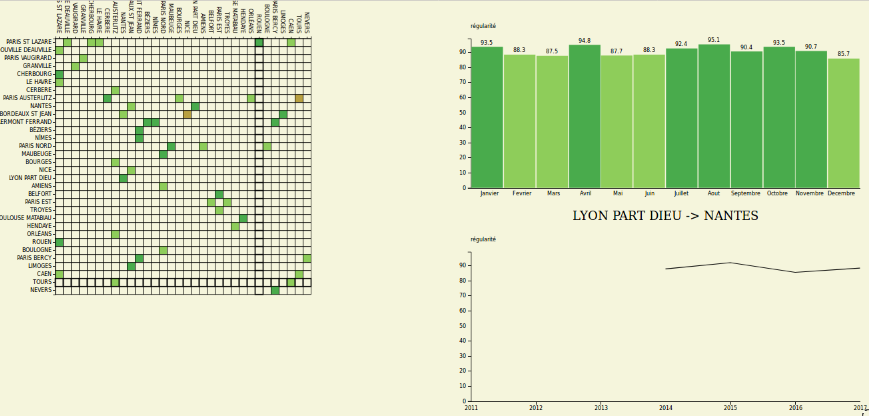
\includegraphics[scale=.5]{intro}]
} 
     
     
\begin{document}


\maketitle

\firstsection{Abstract}
\section{Introduction}
A graph is a way to represent dependencies between entities, each dependencies is represented by an edge between two (or more) vertices. It is a very convenient way to represent many problems in computer science because most of the time we get rid of any combinatorics issues such as exponential complexity and so on. It is also a way to represent real things such as traffic and evolution of things. The main issue with graph is that they are mainly adapted for computers than for human especially when they are very heavy.
\\
\\
\indent
The visualisation of network problematic is now a hot topic in many fields of research such as traffic, cloud computing, scheduling and so on. The Big issue with networks visualisation  is that we do not visualise a big network the way we visualise a small one, we do not visualise a thick network the way we visualise a light one, or a directed one. There is such a high variety of graphs and there is no ready to wear only made-to-measure. But this article will expose some good methods that we can use for graph representation in order to solve a problematic. In this article we will lean on a question to solve, and try to use the best graph representation methods in order to answer this question. The question is "Are SNCF trains always late?". This problematic is very relevant because it concerns everyone and then we will be able to see if the representation we will use is adapt to a non-computer-scientist public.
The SNCF train networks is a very thick graph so the representation will be adapted to this problematic, this article will show you why the adjacency matrix fits our problematic, why it is very interesting on directed graphs, and how we will deduce some other informations from it.
\\
\\
\indent
Then we will use some barchart representation in order to show the evolution of a specific node in the graph. The user graphical interface will be very user friendly, the user will have to click on any box of the matrix in order to see some informations about the traffic of this specific line.
\section{Related Work}

\subsection{Adjacency Matrix and Matrix de Co-occurence: Les Mis\'erables}
About how we could visualise our data, we thought about adjacency matrix and the Mike Bostock work with co-occurence Matrix, les Mis\'erable\cite{Mis},
see Figure~\ref{fig:mat-co}.
There is some studies that talk about how visualising networks. There is essentially two ways of doing so: adjacency matrix or node-link diagram. Node-link diagram wouldn’t be adapted to our problem because we want to see all the links at the same time and it won’t be as readable as desired but with adjacency matrix, we’ll lose some information so we searched how to resolve this issue.
\begin{figure}[h!]
 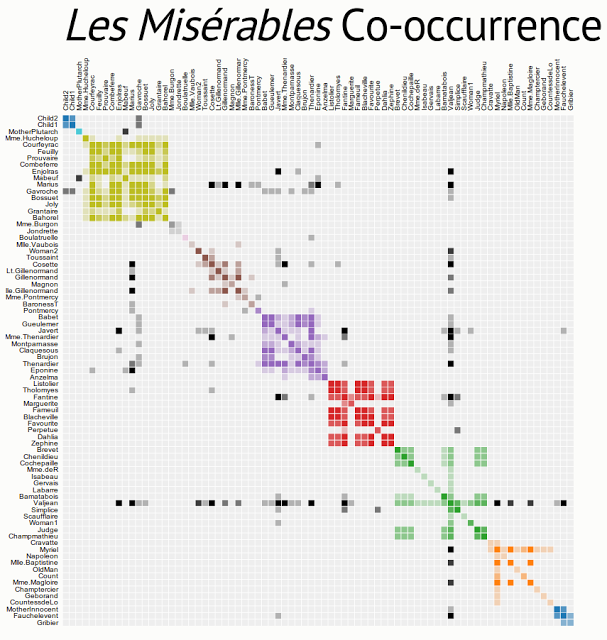
\includegraphics[width=\columnwidth]{mat-co}
 \caption{co-occurence matrix}
 \label{fig:mat-co}
\end{figure} 


\subsection{Juxtaposition}
\indent
As Jean-Daniel Fekete\cite{Fekete} wrote, one drawback of adjacency matrix is that some informations about the topological properties of graphs are lost, as instance, there is no way to represent where Marseille is located to Paris or Lyon or other cities. The juxtaposition of a graph in order to represent the topological aspect of those data must be done if some geographical aspects are correlated. It is also important to notice that adjacency matrix does not provide a way to represent path between multiple nodes as instance the path between Paris, Lyon and Marseille, there will be visualize in a convenient way. As a consequence, if there is no direct path between two cities, there will be no way to represent it. Again, adding a graph or a map of the subject will provide some good support for the visualisation of the problem. 
Now the point is what can we juxtapose next to the adjacency matrix and what additional information this juxtaposed visualisation provides?
\begin{itemize}
\item Barcharts and linecharts: this representation can be a good way to decompose the data over time and then show some evolution of trends.
\item Trendalyzer, if we can correlate different populations of data in order to show a trend, we can use this well known representation.
\item Graph and maps: in order to introduce data in a geographical context graph and maps are required.
\end{itemize}
\section{Projet Description}
\subsection{Data acquisition}
\indent
We choose to work on the delayed train and how to visualize the fact that people thinks that trains are always late. For this project we are using an open dataset from the SNCF website. The dataset is composed of the train station, with traffic regularity rate and the date of the measures. Those data will provide some geographical informations that we must keep in the visualisation of the problem in order to give to the audience concrete results. The exact template of the dataset is: 
the date, the name of the main axis where the train is running, the departure station, the arrival station, the number of trains scheduled, the number of train that runs on this line over the month, the number of train cancelled the number of train delayed, the regularity rate, the number of train on time against the number of train delayed. For our visualisation we have only selected a few of them, which are, the date that we divided on the year and the month, the departure station named source, the arrival station named target and the regularity rate, which is saved as a weight between two stations. We could have added many more that but we wanted to keep our datas simple in order to use the adjacency matrix and the others chart in an effective and simpler way. We lose some accuracy on the datas with only the regularity rate but we think the first and global answer must be simple. We always can add some datas to develop further possibilities in the future.
\\
\\
\indent
Every regularity we saw on the matrix (for each square), is precalculated on a python code before (for the sake of performances) file and added two our cvs, then a year is composed of 12 months numbered form one to twelve, and we also got the month zero which is actually not a month but the mean of each month of the respective year.
For the multiple matrix, on a python code, we created the graph between the stations, and then for each station on the graph we compute the shortest path thanks to dijkstra's algorithm from this station to all the targets. Thus we created the complete graph of each station this representation is much more heavier and is not very relevant of any situation, because when we compute the regularity of a path between two stations, we assume that the delayed train are independants, which is a very naïve assumption. But it's a first step on the vast world of improvements of adjacency matrix.

\subsection{Implementation}
\indent
As explained before, for the sake of performances the main part of the computation are done with python scripts, and save as csv. Then we give the hand to javascript and d3.js module, 
\\
\\
\\
\\
\\
\\
We got two inputs in the javascript, the different stations of the graph and also all the links of the graph [source, target, weight, year, month, comment] so we built the N*N matrix, for the matrix ordering, it is related to the order of the names on the input so we can apply a sort algorithm bases on the links, with this we decided to order the matrix based on the mean of the weight for a specific station. The results are not really relevant, this must need some improvements. The visualisation start in 2011 so the we get all the data gathered during 2011 and we color the matrix in function of the mean of the year. Then the algorithm is waiting for the user to click on a square. Once the user click on a square, the we get all the data comming from this specific train line for this specific year and we draw the barchart month by month. Now the visualisation is waiting for the user to pass his mouse over the months of the barchart in order to display a comment of the problems that the SNCF encountered during this date and also to draw the linechart of the evolution of the traffic quality during this month for every year concerned by the visualisation.
In terms of performances, the multiple train line matrix is quite heavy for the visualisation and it might also be a good point of improvements for the next generation of this algorithm.
\\
\\
\\
\\
\\
\\
\indent
There is three distinct visualisations, each one showing one aspect of the datas that we thought would be interesting. You can chose the year thank to a slider and which data you want to show tank to radio buttons. The whole visualisation follow a color gradient for the regularity.\\
We have five distinct colors : \\
\indent -deep green : $90\%$ - $100\%$ \\
\indent -light green : $80\%$ - $90\%$ \\
\indent -yellow : $70\%$ - $80\%$ \\
\indent -light red : $60\%$ - $70\%$ \\
\indent -deep red : $50\%$ - $60\%$ 
\\
We made that color choice because there is very little datas that go under $50\%$ and we thought that $75\%$ was already pretty bad. For the regularity that is less than $20\%$, we observed a dull version of the last color, but we’re not sure why.
The first visualisation is an adjacency matrix that show the mean regularity for a year that can be chosen by a slider. To draw the matrix, we need to make a dictionary that take the source combined with the target as identifiant and  the regularity, name weight, as value. Each square of the matrix take the information of this dictionary. A tooltip show the regularity percentile of the square when we are over it and you can click on it to show more information on the right side.
On the right side of the matrix, there is the second and third visualisation.
The second visualisation is a histogram that show the regularity by month of the selectionned month and year. A tooltip show the commentary made about a specific month, when it exists, in order to help understanding why one specific month got a really bad result. The regularity percentile is show above the bars, it gives a more accurate information if we’re interested and it also helps to differentiate a $0\%$ from a missing value (and yes, we have at least one value at $0\%$ in the intercité datas).
When you go over the bar of the histogram, the third and last visualisation get to be used: It’s a line chart that show the summary of the regularity over the years for those specific month and chosen train ride.
\\
\\
\indent
In terms of implementation we also worked on the matrix ordering in order to extract some clusters or some patterns. The main plan was to order the matrix by regularity rate of stations, thus we create an algorithm that sort the matrix in function of the mean of the regularity of each station, but this ordering methods was not very relevant, because most of the line are Paris centered, so there is no real cluster possible, it is more due to the data type than the ideas that sats within. Moreover there must be some better methodes to cluster the matrix with some datamining algorithm but this is way beyond the limits of the possible for this specific project.

\subsection{Scenario}
\indent
The visualisation is available on our webpage, first of all the user have to chose the type of train he wants to visualise and if he wants to include non-direct paths, those options are made for the sake of simplicity, the multiple stations variation  is more like an experiment of the limits of our visualisation model, so if the user wants to have a cristal clear representation of the data which goes to the essentials it is better to chose the simple representation. We could have gathered the TGV and the intercit\'e matrix together but because they are not connected by any station, it is better to keep them separated. For the sake of our scenario he has chosen TGV and simple paths, at this stage the chosen visualisation will appear as a matrix, now the user can chose on the left the departure station and the arrival one on the top, he will have to click on the corresponding square on the matrix. For example our user as chose the line: MARSEILLE ST CHARLES -\textgreater LILLE, now on the top, the regularity barchart will appear for this specific line, each bar represents a month, the color variates from green to red regarding the quality of traffic during this specific months for this specific year. When the user pass over a bar with his mouse, two things will be noticed: A comment of the mains reasons for those delayed train, and on the bottom right corner a line of the variation of this specific month all over the years.

\section{Discussion}
\indent
We did not made any measure of understanding time over a population of people so it's quite hard to talk about the quality of our specific visualisation, (faire des citations des articles sur les matrices d'adjacence, vitesse d'analyse des cobayes) 
In terms of data that we can deduce from the visualisation, obviously the trains are not always late but some informations just jump right to the eyes, as instance, the lines that are not related to paris such as Lille -> Marseille have a low rate of regularity, (ajouter image). Even if the multiple station matrix is quite messy, we can easily see that long train ride are more likely to be affected by a delayed train. 
We also see that the year 2015 were pretty bad in terms of regularity, and the end (June to September) of the year 2017 is disastrous due to some natural disaster and other plethora of incidents.



\section{Possible improvements}

There is many ways of improvements in our visualisation one of them is the implementation of an ordering algorithm for the matrix, we now when to plug it on our code and we already tried one as mentionned before but this specific problematic suffer of a lack of knowledge from our side, there is some articles about this specific subject which deals with some common algorithm bases on clumn and line swapping.\cite{visu_reseaux}
We also didn't lean too much on those problematic because they were no good way to order the TGV matrix in a good clustered way, because most of the lines are centered on Paris, so this might algo be a way of improvements, int the data acquisition we can add some other stations such as intercité with the TGV and then each region of france will represent a cluster of intercité trains and thos clusters are connected together by the TGV. This part is really challenging because it needs a lot of data gathering and maybe the matrix would have been too big so we would have been forced to use the nodeTrix method mentionned in the article of Mr Fekete(sitation mise en forme jd fekete). Now we have a good knowledge of adjacency matrix, we will be able to add some new features such as other data like deleted trains instead of delayed ones, or maybe some prediction of the future of the traffic quality with the same visualisation.
In the multiple path problematic, the dijkstra algorithm is very naïve because nobody take more than one TGV during a train travel, but this idea is good to keep and to improve by adding intercité trains in the TGV graph in order to have an accurate visualisation. Moreover for multiple station lines, we considered that delayed trains are independents to one another, but this is very naïve, as instance during strikes or when a train delaye all the other one in the line.
\section{Conclusion}
To conclude, there are several ways to represent flows in traffic network, we have chosen one that is free from any geographical representations, this choice was made because we didn't wanted the user to focus on the distance or the position but only on traffic quality, everything one the visualisation is made for it, as instance, the juxtaposition methods is a way to represent data over time, once the user chose a square in the matrix everything is made for giving as much information as possible about the quality of traffic on this line over the year, with comments about the reasons of somes delayed or problems. We think this webpage is a real success and with thurther works on ordering and data gathering, it can be use by any companie or people that deals with problems on thick traffic graph representation over the time.

\begin{figure}[h!]
 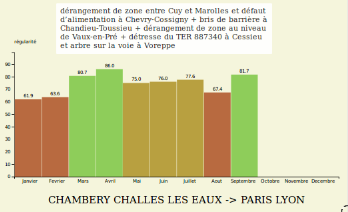
\includegraphics[width=\columnwidth]{comm}
 \caption{commentary}
 \label{fig:comm}
\end{figure}
\begin{figure}[h!]
 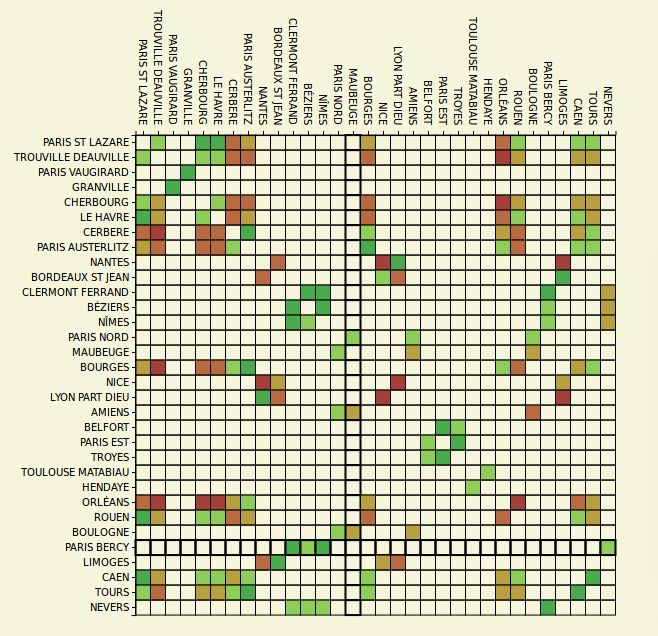
\includegraphics[width=\columnwidth]{intermul}
 \caption{multiple}
 \label{fig:intermul}
\end{figure}
\begin{figure}[h!]
 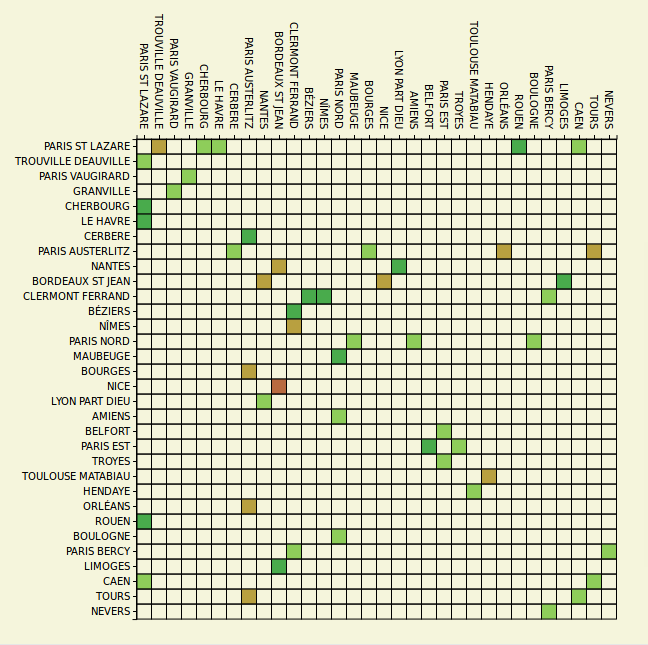
\includegraphics[width=\columnwidth]{intersimp}
 \caption{simple}
 \label{fig:intersimp}
\end{figure}
\begin{figure}[h!]
 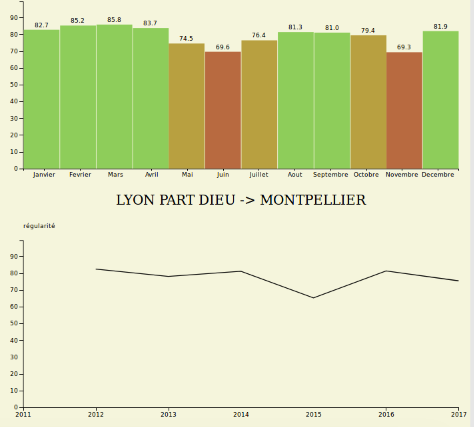
\includegraphics[width=\columnwidth]{hist_line}
 \caption{linechart}
 \label{fig:hist_line}
\end{figure}
\begin{comment}
\indent
The adjacency matrix representation:
In order to solve the problematic, the main idea is to visualise the network train station by train station. With the adjacency matrix, each station will be represented in a line and in a column and for every existing train line between two stations, the corresponding square will be colored regarding the quality of the traffic, see next paragraph. As instance, where the line Marseille collide with the line Lille, we color the square with the right color. Thus, when all this representation is done, every line between station will be color regarding the quality of traffic. Now it is quite important to notice that an A to B line is different than a B to A line we will have some differences in the quality of traffic, and those differences will jump right to the eyes of the public.
(show matrix picture)
The choice of colors:
The color choice is very simple, good is represented by the green color and the worst it gets, darker the red will be. As instance, the line Marseille Lille is getting worst all over the years, so you can see in the representation that each month the green is becoming more and more red. This choice of color is due to the fact that red means bad for everyone and green means good, it also remind traffic lights so it's a good choice of color for this kind of problematic.
(article des premiers \`a \^etre pass\'es)
The barchart representation:
When we click on a specific square, one which represent a line between two stations, some additional data are gathered. Thus we are able to represent the evolution of traffic quality month by month all over the year. this representation is very user friendly because it's simple to use, the user will have to click on the lines he is interested on, Moreover, the informations is hidden until the user wants to learn more about a specific line. And we have some additional we the user puts his cursor on a specific month, there is a feedback on the reason why traffic was delayed during this specific month.
Many way to sort the matrix, many way to visualise:
\end{comment}
\bibliographystyle{plain}
\bibliography{mybib}

\end{document}